\documentclass[a4paper,11pt]{myreport}
%\documentclass{scrreprt}

\usepackage[dvipsnames]{xcolor}
\definecolor{souris}{gray}{0.19}
\definecolor{tagada}{RGB}{35,0,35}
\colorlet{bordeaux}{red!75!blue!25!darkgray}
\usepackage[hyperfootnotes=false]{hyperref}
\usepackage[toc,page]{appendix} 
\usepackage[utf8]{inputenc}
\usepackage[T1]{fontenc}
\usepackage{geometry}
\usepackage[export]{adjustbox}
\geometry{left=75pt,right=75pt,bottom=75pt}
\usepackage{a4wide}
\usepackage[francais]{babel}
\usepackage[babel=true]{csquotes} % csquotes va utiliser la langue définie dans babel
\usepackage{graphics}
\usepackage{movie15}
\usepackage{graphicx}
\usepackage{verbatim}
\usepackage{listings}
\usepackage[capbesideposition=bottom]{floatrow}
%\floatsetup{capposition=bottom}
\usepackage{caption}
\usepackage{color}
\usepackage{fancyhdr}
\usepackage[bottom]{footmisc}


\pagestyle{fancy}
\renewcommand{\footrulewidth}{1pt}
\fancyfoot[C]{\textbf{page \thepage}} 
\fancyfoot[L]{Projet 2A Informatique}
\fancyfoot[R]{Emmanuel Breton\--\--Belz}
\renewcommand{\footrulewidth}{0.7pt}
%\usepackage{syntonly}
%\newenvironment{DocStage}
%\syntaxonly
%%\setlength{\oddsidemargin}{dim souhaitée}
%%\setlength{\evensidemargin}{dim souhaitée}
%%\setlength{\textwidth}{dim souhaitée}
%%\setlength{\headheight}{dim souhaitée}
%%\setlength{\topmargin}}{dim souhaitée}
%%\setlength{\footskip}{90pt}

\setcounter{tocdepth}{2}
 \hypersetup{	
colorlinks=true, %colorise les liens 
breaklinks=true, %permet le retour à la ligne dans les liens trop longs 
urlcolor= blue, %couleur des hyperliens 
linkcolor= tagada ,	%couleur des liens internes 
citecolor=back,	%couleur des références 
pdftitle={Rapport de projet 2A}, %informations apparaissant dans 
pdfauthor={Emmanuel Breton\--\--Belz}, %les informations du document 
pdfsubject={Projet 2A}	%sous Acrobat. 
} 
\title{Jeu vidéo pédagogique utilisant la technologie Oculus VR}
\author{Emmanuel Breton\--\--Belz}


\begin{document} % ------------------------begin---------------------------------------
\def\siecle#1{\textsc{\romannumeral #1}\textsuperscript{e}~si\`ecle}

%reglages pour l’insertion de code
\lstset{language=Java,
basicstyle=\normalsize, % ou ça==> basicstyle=\scriptsize,upquote=true,
aboveskip={1.5\baselineskip},
columns=fullflexible,
showstringspaces=false,
extendedchars=true,
breaklines=true,
showtabs=false,
showspaces=false,
showstringspaces=false,
identifierstyle=\ttfamily,
keywordstyle=\color[rgb]{0,0,1},
commentstyle=\color[rgb]{0.133,0.545,0.133},
stringstyle=\color[rgb]{0.627,0.126,0.941},
}
\nopagebreak[3]


%\maketitle -------------------------------- premiere page
%%\setlength{\textheight}{28cm}
%%\setlength{\topmargin}{-5pt}

\makeatletter

  \begin{titlepage}
  \centering
      {\large \textsc{école nationale supérieur d'ingénieurs de caen}}\\
      \textsc{Dans le cadre du projet 2A}\\
    \vspace{1cm}
    \vspace{1cm}
      {\large\textbf{	\@date\\
      \LARGE{Rapport projet de 2\up{ème} année}}}
      
    \vfill
      
\includegraphics[width=0.25\textheight,center]{./images/LogoEnsicaenSansTexte.jpg}
    \vfill
       {\LARGE \textbf{\@title}} \\
    \vspace{1em}
        {\large \@author} \\
    \vfill

        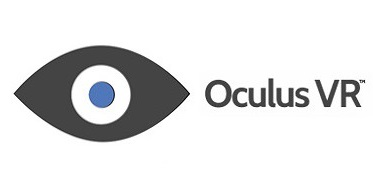
\includegraphics[width=0.25\textheight,left]{./images/oculus_logo.jpg}
        
\includegraphics[width=0.25\textheight,right]{./images/Unity_3D_logo.png}

  \end{titlepage}
\makeatother
%\end --------------------------------------------------------------------

%table des matières :
\setlength{\textheight}{26cm}
\setlength{\topmargin}{-2cm}

\tableofcontents


\listoffigures
\section*{Remerciements}
Tout d'abord je tiens à remercier M. Lebrun pour nous avoir proposer le projet. Nous avoir fourni de la documentation et avoir prêter l'oculus pendant plusieurs semaine pour le prendre en main.
\chapter{Introduction}
\par Le projet Oculus VR consiste en la réalisation d'un jeu à but pédagogique. Destiné à la promotion de l'école lors des journées portes ouvertes et des journées de l'étudiant en fin d'année 2015.
\par La réalisation du projet comprend l'utilisation de la technologie de réalité augmenté \lq\lq{Oculus VR V2} détenu aujourd'hui par le groupe Facebook. Le modèle d'essaye appartient au laboratoire de recherche de l'ENSICAEN. Prêté pour le projet par Gilles Lebrun lors de nos tests.
\begin{figure}[h]
	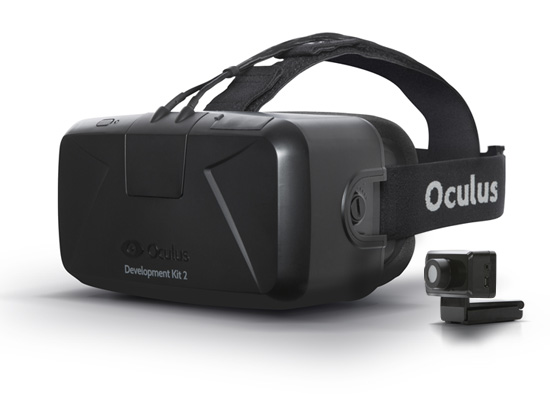
\includegraphics[scale=0.70]{./images/dk2-product.jpg}
	\caption{Casque Oculus VR kit de developpement version 2}
\end{figure}
\chapter{Contexte}
\par Aujourd'hui les jeux vidéos étant un média incontournable, beaucoup de société s'oriente vers l'utilisation de ceux si pour promouvoir, divertir, instruire le grand public. Notre projet ce situe entre le ludisme et la pédagogie et évidement, doit promouvoir en un sens, les compétences acquises lors de la formation à l'école.
\par Pour ce faire nous avons accès à une technologie remise au goût du jour il y a 3 ans, grâce à une campagne Kickstarter : La réalité augmentée.

\chapter{Réalisation}
\section{Outils}
\section{Composants}
\chapter{Difficultés}

\chapter{Résultats}

\chapter{Apports personnel}

\chapter{Glossaire}

\chapter{Annexes}

\begin{figure}[h]
	
\includegraphics[scale=0.70]{./images/LogoEnsicaenSansTexte.jpg}
	\caption{JDialog permettant le réglage d'une LED 4 couleurs}
\end{figure}

\end {document}
